\chapter{Background Information}\label{chapter:background}

\section{Cosmic rays and air showers}

\textbf{What are cosmic rays?}

\textbf{How do cosmic rays relate to water Cherenkov detectors?}

\textbf{How do cosmic rays produce muons and neutrinos?}

\textbf{What are the properties of the muon and neutrino fluxes we need to be concerned with?}

Cosmic rays are high-energy protons and atomic nuclei that propagate through space.
Some of these particles originate from our own sun, and within the Milky Way.
However, cosmic rays have been observed in excess of $\SI{1e20}\eV$.
At these energies, cosmic rays cannot be sufficiently bound by the galactic magnetic field to produce an isotropic flux.
Thus, cosmic rays at this energy scale must either point towards nearby accelerators or arrive roughly isotropically from extra-galactic sources.
The spectrum and spatial distribution of this highest energy population has been shown be distinct from the lower energy population and likely to be of extra-galactic origin.
The sources and acceleration mechanisms of these extra-galactic cosmic rays are unknown to date, and remain a subject of significant study and interest.
Similarly, the sources of lower energy cosmic rays remain unknown despite their possible galactic origin.
Cosmic rays can be observed interacting in the Earth's atmosphere, as they produce extensive particle air-showers whose constituents and products can be observed with a wide range of techniques.
The charged particle products of these interactions have been observed as early as 1912~\cite{hess1912uber}.
These air showers are of particular concern to neutrino detectors as they produce high-energy muons and neutrinos in relative abundance, both of which can be observed by neutrino detectors even with significant shielding and overburden.

When cosmic rays interact with the atmosphere some nuclear fragments can be produced, but the hadronization occurs due to the high energy of the interaction initiating a hadronic particle shower.
Pions and kaons produced in the air shower subsequently decay or interact in the low-density atmosphere.
Leptonic and semi-leptonic decays of charged pions and kaons that produce muons or neutrinos have a large decay branching fraction, resulting in an abundance of muons and neutrinos in any air shower that begins hadronically.
Muons produced in these air showers reach the ground where they can be detected, and often penetrate many kilometers into the Earth's surface.
Neutrinos have an interaction cross section that is approximately a factor of $10^6$ smaller than that of muons, meaning they not only reach the ground but are likely to pass through the Earth without interacting and can be observed by neutrino detectors coming from all directions.

\begin{figure}
	\centering
	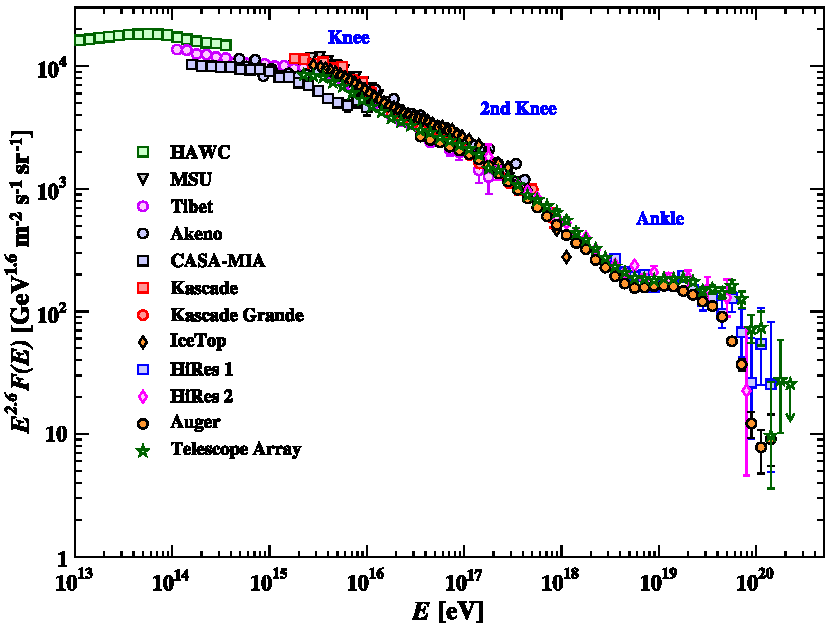
\includegraphics[width=\linewidth]{figures/cosmic_ray_spectrum}
	\internallinenumbers
	\caption{\textbf{\textit{Cosmic Ray Spectrum}}
		This figure is reproduced here from~\cite{PhysRevD.98.030001}.
	}\label{fig:cosmic_ray_spectrum}
\end{figure}

\textbf{Make a diagram of a prototypical cosmic ray air shower.}

\textbf{Find a good reference for the cosmic ray flux so that we can copy a plot here.}

\textbf{Find a good reference or references for the calculation of the neutrino and muon fluxes from cosmic rays.}

\textbf{Discuss the rate of muons at the Earth's surface.}

The flux of cosmic ray

\subsection{Neutrinos in cosmic ray air showers}

\subsection{Muons in cosmic ray air showers}

\section{Neutrino interactions and detection}

Neutrinos are the only neutral leptons in the standard model of particle physics.
Although fundamentally neutrinos only interact through gravity and the exchange of weak bosons, there exist a wide range of processes that dominate the relevant physical behavior of neutrinos at different energy scales.
Such interactions include: nuclear capture, inverse beta-decay, quasi-elastic scattering, resonant particle production, coherent elastic scattering, deep inelastic scattering (DIS), and ultra-high energy interactions~\cite{Vannucci:2017rqs,Akimov:2017ade}.
Above $\si\TeV$ neutrino energies however, only two known processes remain relevant for detection: DIS and resonant $W$ production.
Deep inelastic scattering refers to processes that probe the fundamental components of hadrons.
For neutrinos, this means the exchange of a weak boson with a quark.
The momentum imparted to the quark will produce a hadronic cascade of secondary particles.
The details of the lepton side of the interaction depend heavily on the species of incident neutrino and weak boson exchanged.
We can divide these DIS interactions into two categories based on the weak boson exchanged.
Interactions involving the exchange of a $Z$ are referred to as ``neutral current'' (NC), and those exchanging a $W$ are referred to as ``charged current'' (CC).
Modern techniques for observing neutrino interactions rely on detecting the charged particle products of the initial interaction.
As a consequence of this, the observable energy can be very different for NC and CC events.
Both interactions produce a hadronic cascade, but on the leptonic side of the interaction NC event have an outgoing neutrino (not observable) while CC events have an outgoing charged lepton (observable).
These two interactions are shown in \reffig{fig:DIS}.

\begin{figure}
	\centering
	\begin{tikzpicture}
	\begin{feynman}
	\vertex (a);
	\vertex [below=of a] (b);
	\vertex [above left=of a] (c) {\(\nu_{l} / \overline \nu_{l}\)};
	\vertex [above right=of a] (d) {\(\nu_{l} / \overline \nu_{l}\)};
	\vertex [below left=of b] (e) {\(u/d\)};
	\vertex [below right=of b] (f) {\(u/d\)};
	\diagram* {
		(c) -- [fermion] (a),
		(a) -- [fermion] (d),
		(e) -- [fermion] (b),
		(b) -- [fermion] (f),
		(a) -- [boson, edge label=\(Z^0\)] (b),
	};
	\end{feynman}
	\end{tikzpicture}
	\begin{tikzpicture}
	\begin{feynman}
	\vertex (a);
	\vertex [below=of a] (b);
	\vertex [above left=of a] (c) {\(\nu_{l} / \overline \nu_{l}\)};
	\vertex [above right=of a] (d) {\(l^\pm\)};
	\vertex [below left=of b] (e) {\(u/d\)};
	\vertex [below right=of b] (f) {\(d/u\)};
	\diagram* {
		(c) -- [fermion] (a),
		(a) -- [fermion] (d),
		(e) -- [fermion] (b),
		(b) -- [fermion] (f),
		(a) -- [boson, edge label=\(W^\pm\)] (b),
	};
	\end{feynman}
	\end{tikzpicture}
	\caption{The neutrino deep inelastic scattering processes NC (left) and CC (right) in matter is shown in the figure above for interactions with nucleon component quarks.
	In both cases, significant momentum can be imparted to the outgoing quark which will result in the production of a hadronic particle cascade.
	In NC interactions, only the hadronic cascade may be detectable as the interaction product is a neutrino which is unlikely to undergo another interaction within the detection medium.
	Interactions of the CC variety on the other hand, produce a charged lepton in addition to the hadronic cascade.
	This charged lepton can also be detected if it receives enough energy.}
	\label{fig:DIS}
\end{figure}

The third interaction relevant above $\si\TeV$ neutrino energies is the resonant production of a $W$ boson, otherwise known as the Glashow resonance (GR)~\cite{Glashow:1960zz}.
In matter on Earth this process occurs when an anti-electron neutrino combines with an atomic electron to produce an on-shell $W^+$ as shown in~\reffig{fig:glashow}.
If we consider the rest frame of the electron, then this resonance occurs at a neutrino energy of $\SI{6.3}\PeV$.
For atomic electrons we should consider the rest frame of the atom, and in this case there is a Doppler broadening of the resonance of $\sim\SI{20}\percent$ due to the orbital motion of the electrons~\cite{Loewy:2014zva}.
In practice this broadening is small in comparison to the energy resolution of modern neutrino detectors that have access to this energy scale, and any further broadening from thermal motion will be even smaller.
The production of a $W^+$ and it's subsequent decay can result in either a hadronic shower similar to a NC interaction, or a leptonic final state similar to a CC interaction.
These two possibilities correspond to the hadronic and leptonic decay modes of the $W$ respectively.

\begin{figure}
	\centering
	\begin{tikzpicture}
	\begin{feynman}
	\vertex (a);
	\vertex [right=of a] (b);
	\vertex [above left=of a] (c) {\(\overline \nu_{e}\)};
	\vertex [below left=of a] (d) {\(e^-\)};
	\diagram* {
		(c) -- [fermion] (a),
		(a) -- [fermion] (d),
		(a) -- [boson, edge label=\(W^+\)] (b),
	};
	\end{feynman}
	\end{tikzpicture}
	\caption{The production of an on-shell $W^+$ boson through the combination of an anti-electron neutrino and electron.
	This resonant process occurs at neutrino energies around $\SI{6.3}\PeV$.}
	\label{fig:glashow}
\end{figure}

Through either a NC interaction or the hadronic decay of a $W$ boson, neutrinos can induce a hadronic shower.
In a hadronic shower, both charged hadrons and leptons are produced which can be detected through well established methods.
Charged current interactions produce a hadronic shower by imparting momentum to a quark which is then hadronized, although the charged lepton produced in the interaction is also detectable and can significantly alter the detection signature of the event.

Through either a CC interaction or the leptonic decay of a $W$ boson, neutrinos can produce a detectable charged lepton, although the detection signature differs depending on the flavor of charged lepton produced.
Focusing on dense detection media like ice or water, the detection signatures of the three flavor of charged lepton are as follows.
High energy electrons and positrons immediately interact with the detection media to initiate an electromagnetic cascade where charge leptons and high energy photons are alternately produced by one another.
This electromagnetic cascade develops in a roughly spherical fashion within the dense detection medium, but has a directional bias because of the momentum of the first charged lepton.

Muons from high energy neutrino interactions do not interact as readily as electrons and positrons due to their larger mass.
Instead, muons are able to travel several kilometers in dense media before eventually losing enough energy that they quickly decay.
Along their entire path length, muons lose energy by interacting with the detection medium.
These ``energy loss'' interactions include ionization, electron-positron pair production, bremsstrahlung, and photo-nuclear interactions.
Although these processes are highly stochastic, the average energy loss of muons approximately follows $-dE/dx=a+bE$ where $a$ is determined by the ionization energy losses and $b$ is defined by the other processes.
In general $a$ and $b$ and both functions of the muon energy $E$, but this linear approximation where $a$ and $b$ are constant holds locally as both are slowly varying as a function of $E$.
For muon energies above $\SI{1}\TeV$, the so called ``radiative'' term $bE$ dominates the average energy losses.
Figure~\ref{fig:energy_losses} shows the energy loss rate for the different processes.
Once the radiative losses have taken over above $\sim\SI{1}\TeV$, the losses grow exponentially with energy.

\begin{figure}
	\centering
	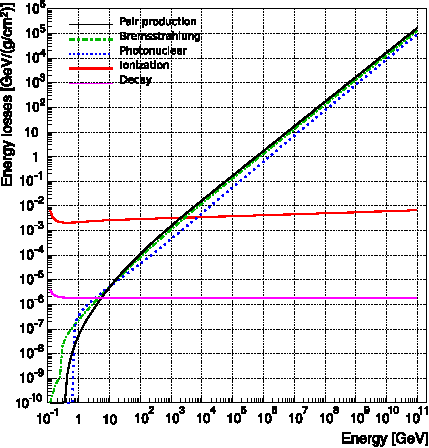
\includegraphics[width=\linewidth]{figures/energy_losses}
	\internallinenumbers
	\caption{\textbf{\textit{Muon Energy Losses}}
		The muon energy loss rate computed for water is plotted as a function of the muon energy for the five different loss processes.
		This figure is reproduced here from~\cite{Koehne:2013gpa}.
		Radiative energy losses dominate above $\sim\SI{1}\TeV$.
		Although it is a smaller contribution to the energy losses, photo-nuclear interactions are the main source of uncertainty above $\sim\SI{1}\TeV$.
	}\label{fig:energy_losses}
\end{figure}

The strong dependence of the energy loss rate on muon energy means that the energy lost while traversing the detector can be used to estimate a muon's energy.
For simple observables like the total energy lost over $\SI{1}\km$ the stochastic energy losses introduce large variations between muons of the same energy, reducing their power as a proxy for the muon energy.
Figure~\ref{fig:muon_energy} shows the energy of muons lost within $\SI{1}\km$ of ice; a distribution with very long tails.
In practice the muon energy can currently be determined to within a factor of $2$, however improved techniques that take advantage of more detailed information may achieve a resolution as small as $\SI{10}\percent$ in the future.

\begin{figure}
	\centering
	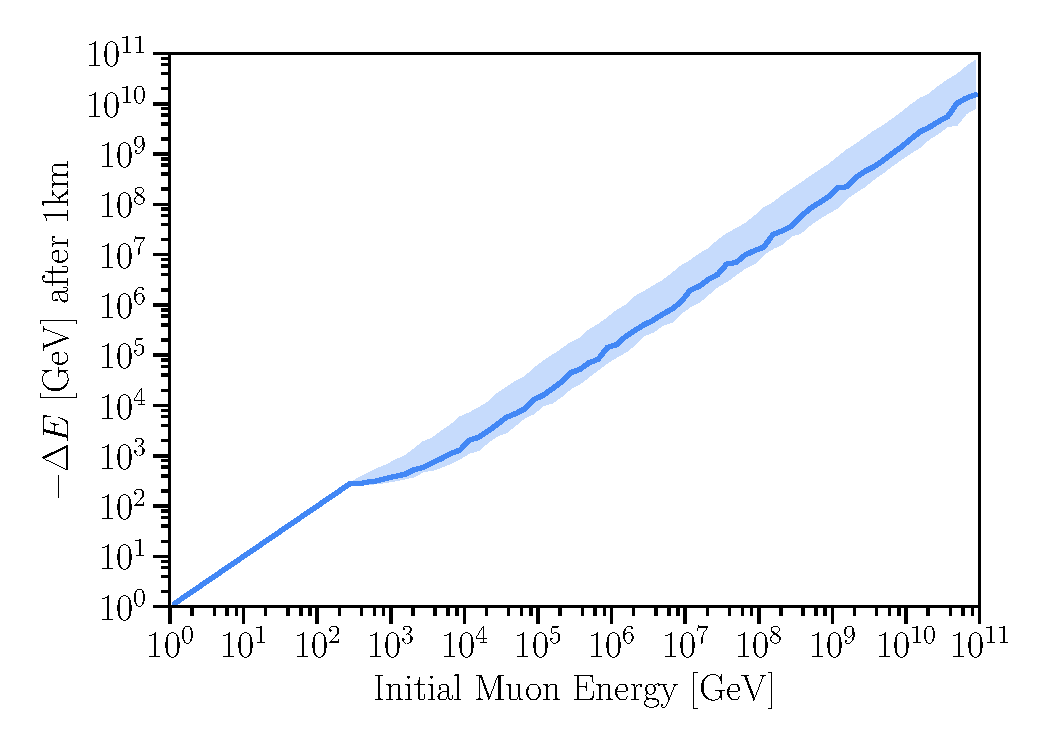
\includegraphics[width=\linewidth]{figures/muon_energy}
	\internallinenumbers
	\caption{\textbf{\textit{Muon energy loss in $\SI{1}\km$ of ice.}}
	Muons are propagated through $\SI{1}\km$ of ice, and their lost energy recorded.
	For each initial muon energy, the MAP and $\SI{90}\percent$ HPD are plotted here.
	There is a strong correlation between the initial energy and energy lost.
	However, the distribution has very long tails, making a precise determination of the muon energy based on this observable impossible.
	}\label{fig:muon_energy}
\end{figure}

Taus produced through a CC interaction or the leptonic decay of a $W$ boson are also detectable.
The short decay length of a tau, $\SI{50}\meter / \si\PeV$, means it is likely to decay very close to the neutrino interaction vertex.
Taus decay hadronically with a branching ratio of $\SI{64.79}\percent$, which results in a hadronic shower.
Leptonic decay modes of the tau are decay to a charged lepton and corresponding neutrino of either electron or muon flavor.
In the electron case, an electromagnetic shower results; whereas in the muon case a far traveling muon is produced.
For taus produced via the decay of a $W$ boson, the event is indistinguishable from taus produces via CC and NC interactions other than by resonance energy at which this process occurs.
Although a tau may traverse tens of meters, which is detectable by IceCube, the energy losses are still negligible over these distances.

From the wide variety of methods for detecting charged particles, water Cherenkov detectors are most common for detecting neutrinos in this high-energy regime above $\SI{1}\TeV$.
Water Cherenkov detectors have the advantage that their detection medium is both abundant and inexpensive, a major motivator in the design of IceCube.
Cherenkov radiation is the result of charged particles propagating through a dielectric medium faster than the phase velocity of light.
As charged particles pass through dielectric material, the ionization of the medium induces the emission of light.
For particles faster than the phase velocity, the emission forms a conical coherent wave front at a well defined angle to the particle's path.

\begin{figure}
	\centering
	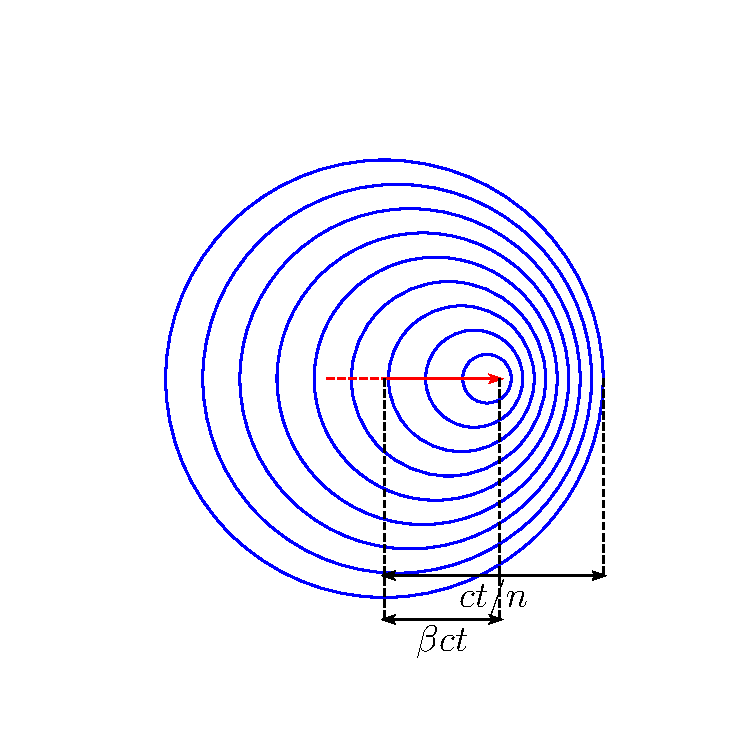
\includegraphics[width=0.45\linewidth]{figures/no_cherenkov}
	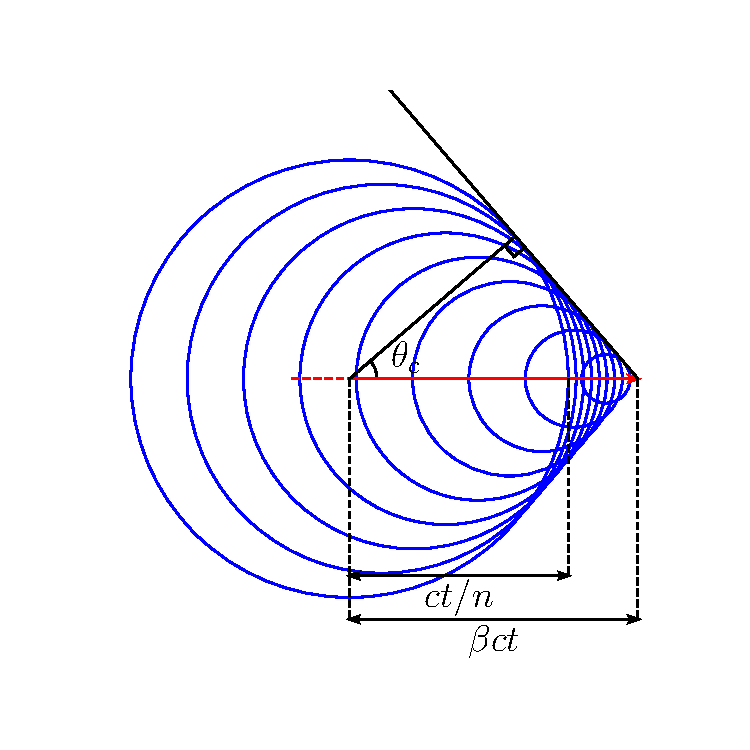
\includegraphics[width=0.45\linewidth]{figures/cherenkov}
	\internallinenumbers
	\caption{\textbf{\textit{Cherenkov radiation.}}
		This diagram shows the photon wave fronts as a charged particle moves through a dielectric medium.
		On the left for $\beta < 1/n$ and on the right for $\beta \geq 1/n$.
		The Cherenkov angle $\theta_c$ is shown on the right, and describes a ray perpendicular to the coherent wave front.
	}\label{fig:cherenkov}
\end{figure}


These detectors use Cherenkov radiation to detect particles, but the high-energy secondary charged leptons themselves do not produce many Cherenkov photons.
Most of the Cherenkov photons are produced by the tertiary particle showers that these leptons give rise to when they lose energy in the detection medium.
This increased light-yield allows detectors to be sparsely instrumented while maintaining detection efficiency and reconstruction quality.

Water Cherenkov detectors often make use of photo-multiplier-tubes (PMTs) to detect Cherenkov photons.
PMTs have a thin photo-cathode that is held at a high-voltage differential with respect to an anode; this allows the production and acceleration of a photo-electron when photons pass through the photo-cathode.
Accelerated photo-electrons hurtle towards an amplification stage composed of many dynodes, each held at a large voltage difference to the adjacent dynodes.
This setup allows a single photo-electron to produce many secondary electrons upon interaction with a dynode, starting an exponential cascade of electrons across the dynode stages.
The resulting cascade of electrons is amplified with respect to the original signal enough that they can be detected electronically as a voltage change.
In this way, PMTs can be sensitive to single photons, provided one is able to reach the photo-cathode.